\section*{Tulokset}

\subsection*{Laadulliset tulokset}

\emph{Atlas ti-} ohjelman avulla tuotettu tekstien koodaus tuotti
tavallaan selkeän tuloksen: konstruktivistis/diskurssianalyyttiset ja
realistiset työt erosivat sisällöltään toisistaan erityisesti
tutkimusmenetelmien kuvauksessa. Konstruktivistisiin töihin liittyi
usein episteemisen relativismin mukainen tarina siitä, kuinka
\emph{totuutta ei ole olemassa}, ja että todellisuutta koskevat
tulkinnat ovat kieleen sidottuja. Opinnäytteissä käytettävä
argumentaatio on hyvin samankaltaista kuin yliopistojen pro
gradututkielmissa. Vastaavasti realistisissa töissä viitattiin usein nk.
\emph{CMO-kaavaan}, jonka mukaan projektin tai intervention
vaikuttavuutta voidaan tarkastella vain kontekstissaan.

\subsection*{Rakennemallinnuksen tulokset}

Spektraalinen mallinnus tuotti 10 aihealueen erottelun (15 iteraatiota).

\begin{enumerate}

\item Topic : lapsi, vanhempi, päiväkoti, asia, toiminta 
\item Topic : vanhempi, lapsi, nuori, perhe, tutkimus 
\item Topic : palvelukeskus, asunnoton, aineisto, kirjoitus, oppilas 
\item Topic : tehdä, suunnitelma, työ, asiakas, tulla  
\item Topic : johtaja, opetus, valmistaa, lapsi, johtajuus 
\item Topic : perhe, perhetyö, lapsi, palvelu, työ 
\item Topic : nainen, väkivalta, työntekijä, mies, väkivaltainen 
\item Topic : asia, kohtaaminen, tutkimus, sosiaalityö, sosiaalityöntekijä  
\item Topic : asiakas, toiminta, palvelu, arviointi, työ 
\item Topic : ryhmä, toiminta, ihminen, asukas, toinen

\end{enumerate}


%%% tähän ensimmäinen kuvio %%%%


\begin{center}
\begin{figure}[ht!]

%\resizebox{5cm}{!}
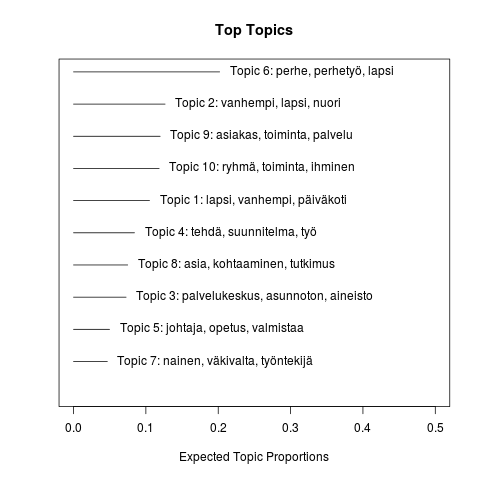
\includegraphics{toptopics.png}

\caption{10 yleisintä topicia}
\label{kuvio1}
\end{figure}
\end{center}


%%%% toinen kuvio, covariate comparison %%%%%


%\begin{center}
\begin{figure}[ht!]

%\resizebox{5cm}{!}
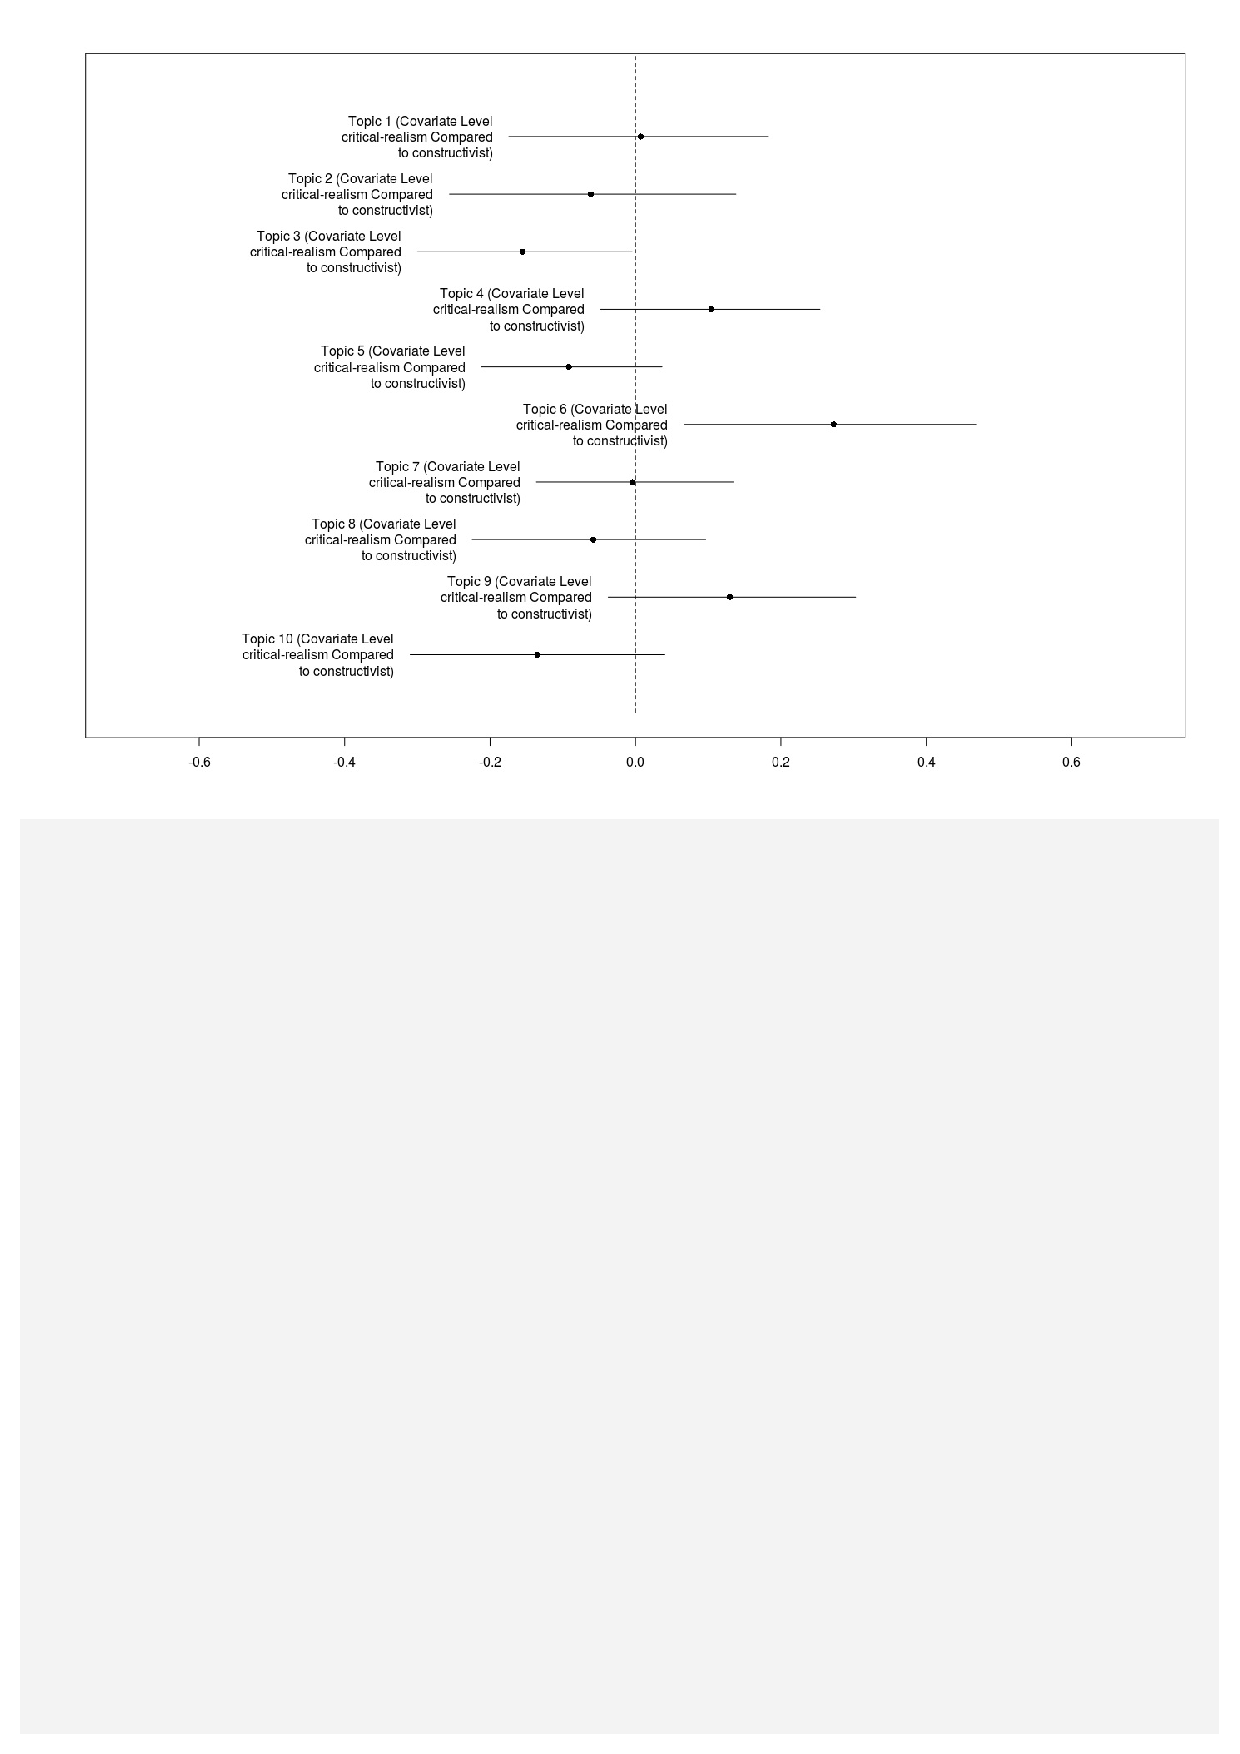
\includegraphics{covariate.pdf}

\caption{10 yleisintä topicia}
\label{kuvio2}
% \addcontentsline{lof}{figure}{}

\end{figure}
%\end{center}

\subsection*{Dokumentit joissa aihe esiintyy}

Topikit jakautuvat niin, että

\begin{itemize}

\item Topicit 9, 6 ja  4: 5 kriittisen realismin ja 1 konstruktionismin ryhmään
  kuuluvaa työtä.

\item Topicit 10 ja 3: 5 konstruktionismin ja 1 kriittisen realismin ryhmään
  kuuluvaa työtä.

\end{itemize}

